\documentclass[10pt]{article}
\usepackage{listings}
\usepackage[utf8]{inputenc}
\usepackage[margin=1in]{geometry} 
\usepackage{amsmath,amsthm,amssymb, graphicx, multicol, array, caption, subcaption}
\usepackage{textcomp}
\usepackage{tikz}
 \lstset{language=Python}    
\newcommand{\N}{\mathbb{N}}
\newcommand{\Z}{\mathbb{Z}}
 \renewcommand{\qedsymbol}{}
 \renewcommand{\figurename}{Fig.}
 \renewcommand{\delta}{\partial}
\newenvironment{problem}[2][Partie]{\begin{trivlist}
\item[\hskip \labelsep {\bfseries #1}\hskip \labelsep {\bfseries #2.}]}{\end{trivlist}}
\begin{document}
 
\title{Simulación: Trebuchet MURLIN}
\author{R. Seguel, J.P. Soto, P. Cuello y M. Bataille}
\date{Mayo y Junio 2016}
\maketitle

\section{Partícula amarrada a un disco}

En esta sección estudiaremos el movimiento de una partícula amarrada a un disco por una cuerda. La situación esta represantada
en la siguiente figura. Tomaremos como condiciones iniciales, $\alpha = \beta = \frac12\pi$.

Para resolver este problema vamos a estudiar el lagrangiano $L$ y, utilizando la ecuación de Lagrange, encontraremos la
ecuación diferencial que resume el movimiento de $B$. Luego, a partir de esta ecuación, determinaremos los valores de los ángulos
para cada instante en un determinado intervalo.
\begin{figure}[h]
\centering

\begin{tikzpicture}
\draw (0,0) circle (2);
\draw[->] (-3,0) -- (3,0);
\draw[->] (0,-3) -- (0,3);
\draw (45:2) node[above left] {$A$};
\draw (45:1.9) -- (45:2.1);
\draw (45:2) ++(2,0) node[below right] {$B$};
\draw (45:2) ++(2,0) node {$\bullet$};
\draw [dashed] (0:0) -- (45:2);
\draw (45:2) -- ++(2,0);
\draw (45:2) -- ++(0,1.5) -- ++(0,-4);
\draw[->] (-90:1) arc (-90:45:1);
\draw (-25:0.6) node {$\alpha$};
\draw[->] (45:2) ++(-90:1) arc (-90:0:1);
\draw (45:2) ++(-45:0.6) node {$\beta$};
\end{tikzpicture}
\caption{Representación de la situación}
\end{figure}
Llamaremos $\ell_A$ el radio del disco, $\ell_B$ el largo de la cuerda y $m_B$ la masa de la partícula $B$.

Primero determinamos las coordenadas de $B$,
\begin{align*}
x_B &= x_A + \ell_B\sin{\beta} \\
	&= \ell_A\sin{\alpha} + \ell_B\sin{\beta} \\
y_B &= y_A - \ell_B\cos{\beta} \\
	&= -\ell_A\cos{\alpha} - \ell_B\cos{\beta}
\end{align*}
Derivando la posición de $B$ en el tiempo encontramos la velocidad,
\begin{align*}
v_B(x) = \dot{x} &= \ell_A\dot{\alpha}\cos{\alpha} + \ell_B\dot{\beta}\cos{\beta} \\
v_B(y) = \dot{y} &= \ell_A\dot{\alpha}\sin{\alpha} + \ell_B\dot{\beta}\sin{\beta}
\end{align*}
Deducimos la expresión de la energía cinética,
y la energía potencial $V$:
\begin{align*}
T &= \frac12m_Bv_B^2 + \frac12I\omega^2 \\
	&= \frac12m_B\left(\ell_A^2\dot{\alpha}^2+\ell_B^2\dot{\beta}^2+ 2\ell_A\ell_B\dot{\alpha}\dot{\beta}\cos{(\alpha-\beta)}\right) + \frac12I\dot{\alpha}^2 \\
V &= m_Bgy_B \\
	&= -m_Bg\left(\ell_A\cos{\alpha} + \ell_B\cos{\beta}\right) \\
L &= T-V \\
 &= \frac12m_B\left(\ell_A^2\dot{\alpha}^2+\ell_B^2\dot{\beta}^2+ 2\ell_A\ell_B\dot{\alpha}\dot{\beta}\cos{(\alpha-\beta)}\right) + \frac12I\dot{\alpha}^2 + m_Bg\left(\ell_A\cos{\alpha} + \ell_B\cos{\beta}\right) \\
\end{align*}
Derivamos el lagrangiano en cada grado de libertad.
\begin{align*}
\frac{\partial L}{\partial \dot{\alpha}} &= m_B\ell_A^2\dot{\alpha}+m_B\ell_A\ell_B\dot{\beta}\cos{(\alpha-\beta)}+I\dot{\alpha} \\
\frac{d}{dt}\left(\frac{\partial L}{\partial \dot{\alpha}}\right) &= m_B\ell_A^2\ddot{\alpha} + m_B\ell_a\ell_B(\ddot{\beta}\cos{(\alpha-\beta)}-\dot{\beta}\sin{(\alpha-\beta)}(\dot{\alpha}-\dot{\beta}) ) + I\ddot{\alpha}\\
\frac{\partial L}{\partial \dot{\beta}} &= m_B\ell_B^2\dot{\beta}+m_B\ell_A\ell_B\dot{\alpha}\cos{(\alpha-\beta)} \\
\frac{d}{dt}\left(\frac{\partial L}{\partial \dot{\beta}}\right) &= m_B\ell_B^2\ddot{\beta} + m_B\ell_A\ell_B(\ddot{\alpha}\cos{(\alpha-\beta)}-\dot{\alpha}\sin{(\alpha-\beta)}(\dot{\alpha}-\dot{\beta})) \\
\frac{\partial L}{\partial \alpha} &= -m_B\ell_A\ell_B\dot{\alpha}\dot{\beta}\sin{(\alpha - \beta)} - m_Bg\ell_A\sin{\alpha} \\
\frac{\partial L}{\partial \beta} &= m_B\ell_A\ell_B\dot{\alpha}\dot{\beta}\sin{(\alpha-\beta)}-m_Bg\ell_B\sin{\beta}
\end{align*}
Aplicamos la ecuación de Lagrange,
\begin{align}
 \frac{\partial L}{\partial \alpha} &= \frac{d}{dt}\left(\frac{\partial L}{\partial \dot{\alpha}}\right) \nonumber \\
 -m_B\ell_A\ell_B\dot{\alpha}\dot{\beta}\sin{(\alpha-\beta)}-m_Bg\ell_A\sin{\alpha} &= m_B\ell_A^2\ddot{\alpha}+m_B\ell_A\ell_B(\ddot{\beta}\cos{(\alpha-\beta)}-\dot{\beta}\sin{(\alpha-\beta)}(\dot{\alpha}-\dot{\beta}))+I\ddot{\alpha} \nonumber \\
 -m_Bg\ell_A\sin{\alpha} &= (I+m_b\ell_A^2)\ddot{\alpha} + m_B\ell_A\ell_B\ddot{\beta}\cos{(\alpha-\beta)} + m_B\ell_A\ell_B\dot{\beta}^2\sin{(\alpha-\beta)} \nonumber\\
 (\frac{I}{m_B}+\ell_A^2)\ddot{\alpha} + \ell_A\ell_B\ddot{\beta}\cos{(\alpha-\beta)} &= -g\ell_A\sin{\alpha}-\ell_A\ell_B\dot{\beta}^2\sin{(\alpha-\beta)}
 \\
  \frac{\partial L}{\partial \beta} &= \frac{d}{dt}\left(\frac{\partial L}{\partial \dot{\beta}}\right) \nonumber \\
  m_B\ell_A\ell_B\dot{\alpha}\dot{\beta}\sin{(\alpha-\beta)}-m_Bg\ell_A\sin{(\beta)} &= m_B\ell_B\ddot{\beta}+m_B\ell_A\ell_B\ddot{\alpha}\cos{(\alpha-\beta)}-m_B\ell_A\ell_B\dot{\alpha}\sin{(\alpha-\beta)}(\dot{\alpha}-\dot{\beta}) \nonumber \\
 -m_Bg\ell_B\sin{\beta} &=m_B\ell_B^2\ddot{\beta}+m_B\ell_A\ell_B\ddot{\alpha}\cos{(\alpha-\beta)}-m_B\ell_A\ell_B\dot{\alpha}^2\sin{(\alpha-\beta)} \nonumber \\
\ell_B^2\ddot{\beta} +\ell_A\ell_B\ddot{\alpha}\cos{(\alpha-\beta)} &= \ell_A\ell_B\dot{\alpha}^2\sin{(\alpha-\beta)} -g\ell_B\sin{\beta}
 \end{align}
 
 Ahora que determinamos las ecuaciones diferenciales, nos queda implementarlas en un programa y resolverlas numéricamente.
 Para resolver estas ecuaciones diferenciales, tenemos que implementar una función tal que, $$\frac{dx}{dt} = f(x) $$

Donde,
 \begin{align*}
x = \begin{pmatrix}
\alpha \\ \beta \\ \dot{\alpha} \\ \dot{\beta} 
\end{pmatrix} && f(x) = \begin{pmatrix}
\dot{\alpha} \\ \dot{\beta} \\ \ddot{\alpha} \\ \ddot{\beta}
\end{pmatrix}
\end{align*} 

Pero, ya conocemos el valor de $\dot{\alpha}$ y $\dot{\beta}$ en función de $x$.
Nos queda entonces determinar la expresión de $\ddot{\alpha}$ y $\ddot{\beta}$ en función de $x$. 

Para determinar estos valores podemos visualizar las ecuaciones $(1)$ y $(2)$ como un producto entre dos matrices

\begin{equation*}
\begin{pmatrix}
A & B \\ C & D
\end{pmatrix}
\begin{pmatrix}
\ddot{\alpha} \\ \ddot{\beta}
\end{pmatrix}
=
\begin{pmatrix}
E  \\ F
\end{pmatrix}
\end{equation*}


Donde,
\begin{tabular}{ccc}
$A = \frac{I}{m_B}+\ell_A^2$ & $B = \ell_A\ell_B\cos{(\alpha-\beta)}$ & $E =-g\ell_A\sin{\alpha} - \ell_A\ell_B\dot{\beta}^2\sin{(\alpha-\beta)}$ \\
$C = \ell_A\ell_B\cos{(\alpha-\beta)}$ & $D = \ell_B^2$ & $F=\ell_A\ell_B\dot{\alpha}^2\sin{(\alpha-\beta)} -g\ell_B\sin{\beta}$\\
\end{tabular}

\vspace{0.2cm}

Para resolver esta ecuación calcularemos el determinante $\Delta$ de la matriz,
\begin{align*}
\Delta &= AD - BC \\
			&= \left(\frac{I}{m_B}+\ell_A^2\right)\ell_B^2 - \ell_A\ell_B\cos{(\alpha-\beta)}\times\ell_A\ell_B\cos{(\alpha-\beta)} \\
            &= \left(\frac{I}{m_B}+\ell_A^2-\ell_A^2\cos^2{(\alpha-\beta)}\right)\ell_B^2 \\
            &= \left(\frac{I}{m_B} + \ell_A^2\sin^2{(\alpha-\beta)}\right)\ell_B^2
\end{align*}

Podemos ver que $\Delta \neq 0$ (es más, $\Delta >0$), por lo tanto la matriz se puede invertir. La solución es entonces,
\begin{equation}
\begin{pmatrix}
\ddot{\alpha} \\ \ddot{\beta}
\end{pmatrix}
=
\frac{1}{\Delta}
\begin{pmatrix}
D & -B \\ -C & A
\end{pmatrix}
\begin{pmatrix}
E \\ F 
\end{pmatrix}
\end{equation}
Fácilmente podemos resolver numéricamente esta ecuación con un algoritmo. Así obtenemos resultados interesantes, 
\begin{figure}[h]
 \centering
 \begin{subfigure}{0.4\textwidth}
  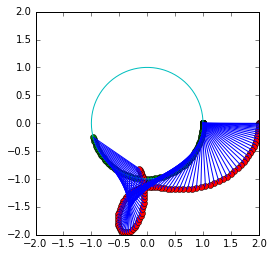
\includegraphics[width=\textwidth]{../fig/fig.png}
  \caption{Caida de la partícula entre 0s y 2s}
 \end{subfigure}
 \begin{subfigure}{0.4\textwidth}
  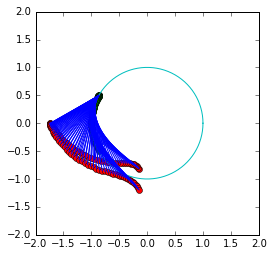
\includegraphics[width=\textwidth]{../fig/fig2.png}
  \caption{Caida de la partícula entre 2s y 4s}
 \end{subfigure}
\caption{Simulación de la caida libre de la particula}

\end{figure}

\section{Implementación del contrapeso}

Hasta ahora hemos logrado modelar el movimiento de una partícula amarrada a un disco. Para acercarnos más a la situación real, tendremos que agregar
el peso que provoca que el disco comience a rotar. Diremos entonces que este peso $P$ se deja caer a una altura inicial $h_0$ sin velocidad inicial. La
cuerda que une el contrapeso al disco (pasando por una polea) tendrá un largo $\ell_P$. Tenemos entonces la situación siguiente,

\begin{figure}[h]
\centering
\begin{tikzpicture}
 \draw (0,0) circle (2);
 \draw (45:2) -- (45:3.5);
 \draw (52:2.75) node {$\ell_P$};
 \draw (58:1.3) node {$\ell_A$};
 \draw[dotted] (0:0) -- (45:2);
 \draw (45:4) circle (0.5);
 \draw (45:4) ++(-90:0.5) -- ++(-90:1);
 \draw (45:4) ++(-90:1.5) node {$\bullet$};
 \draw (45:4) ++(-90:1.5) node[below] {$P$};
 \draw[->] (0,-3) -- (0,4);
 \draw[->] (-3,0) -- (4,0);
 \draw[<->][ultra thin] (1:3.1) -- ++(90:1.3);
 \draw[<->][ultra thin] (1:3.6) -- ++(90:2); 
 \draw (0:3.1) ++(90:0.7) node[right] {$h$};
 \draw (0:3.6) ++(90:1.2) node[right] {$h_0$};
 \draw[->] (-90:0.7) arc (-90:90:0.7);
 \draw[->] (-90:1.5) arc (-90:45:1.5);
 \draw (-35:0.8) node[above left] {$\alpha_0$};
 \draw (-27.5:1.5) node[above left] {$\alpha$};
\end{tikzpicture}
\caption{Representación de la situación}
\end{figure}[h]

A partir de la figura podemos deducir que,

\begin{align*}
 \Delta_h &= \ell_A(\alpha_0-\alpha) \\
 h_0-h &= \ell_A(\alpha_0-\alpha) \\
 h &= h_0-\ell_A(\alpha_0-\alpha)
\end{align*}

O, escrito de otra manera,

\begin{equation}
 y = h_0 - \ell_A(\alpha_0-\alpha)
\end{equation}

A partir de esta expresión, podemos deducir,

\begin{equation*}
 \dot{y} = \ell_A\dot{\alpha}
\end{equation*}

Este sistema está superpuesto al sistema estudiado en la sección anterior. Por lo tanto, la expresión de la energía cinética así como la
energía potencial y el lagrangiano, seran similares. Entonces, definiremos $T'$ de manera que la energía cinética total del sistema corresponde a
$T = T_0 + T'$ donde $T_0$ es la energía cinética del sistema anterior. Lo mismo para $V'$ y $L'$.

Tenemos entonces,

\begin{align*}
 T' &= \frac12 m_Pv^2_P \\
  &= \frac12 m_P\ell_A^2\dot{\alpha}^2 \\
  V' &= m_pg(h_0-\ell_A(\alpha_0-\alpha)) \\
  L' &= \frac12m_P\ell_A^2\dot{\alpha}^2 - m_Pg(h_0-\ell_A(\alpha_0-\alpha)
\end{align*}

Determinamos las derivadas correspondientes,

\begin{align*}
 \frac{\partial L'}{\partial \alpha} &= m_Pg\ell_A \\
 \frac{\partial L'}{\partial \dot{\alpha}} &= m_P\ell_A^2\dot{\alpha} \\
 \frac{d}{dt}\left(\frac{\partial L'}{\dot{\alpha}}\right) &= m_P\ell_A^2\ddot{\alpha} 
\end{align*}

Introducimos estos resultados en la ecuación $(1)$,

\begin{align}
  \left(\frac{I}{m_B}+\ell_A^2+\frac{m_P}{m_B}\ell_A^2\right)\ddot{\alpha} + \ell_A\ell_B\ddot{\beta}\cos{(\alpha-\beta)} &= -\frac{m_P}{m_B}\ell_A\left(\ell_A\dot{\alpha} + g\right)-g\ell_A\sin{\alpha}-\ell_A\ell_B\dot{\beta}^2\sin{(\alpha-\beta)}
\end{align}

A partir de esto, actualizamos los valores en la matriz,

\begin{align*}
 A = \frac{I}{m_B}+\ell_A^2+\frac{m_P}{m_B}\ell_A^2 && E = -\frac{m_P}{m_B}\ell_A\left(\ell_A\dot{\alpha} + g\right)-g\ell_A\sin{\alpha}-\ell_A\ell_B\dot{\beta}^2\sin{(\alpha-\beta)}
\end{align*}

Calculamos el determinante,

\begin{align*}
 \Delta &= \left(\frac{I}{m_B}+\ell_A^2+\frac{m_P}{m_B}\ell_A^2\right)\ell_B^2 -\ell_A^2\ell_B^2\cos^2{(\alpha-\beta)} \\
	&= \left(\frac{I}{m_B}+\ell_A^2\sin^2{(\alpha-\beta)}+\ell_A^2\frac{m_P}{m_B}\right)\ell_B^2
\end{align*}

De nuevo, podemos ver que $\Delta \neq 0$. Así, solo tenemos que cambiar los valores de $A$, $E$ y $\Delta$  para obtener la solución numérica para
este sistema.

\end{document}